\externaldocument{chapter5}
\chapter{Automated Discovery of Failure Domain}
\label{chap:ADFD}
%\ifpdf
%    \graphicspath{{chapter4/AdfdFigs/PNG/}{chapter4/AdfdFigs/PDF/}{chapter4/AdfdFigs/}}
%\else
 %   \graphicspath{{chapter4/AdfdFigs/EPS/}{chapter4/AdfdFigs/}}
%\fi

\section{Introduction}\label{sec:intro5}
Testing is a fundamental requirement for assessing the quality of any software. Manual testing is labour-intensive and error-prone; therefore, automated testing is often used which significantly reduces the cost of software development and its maintenance~\cite{beizer1995black}. Most of the modern black-box testing techniques execute the SUT with specific input and results obtained are compared against the test oracle. A report is generated at the end of each test session depicting any discovered faults and the input values which triggers the failures. Developers fix the discovered faults in the SUT with the help of these reports. The revised version of the system is given back to the testers to find more faults and this process continues till the desired level of quality already set in the test plan is achieved or the provided resources are exhausted~\cite{parnin2011automated}.

%The fact that exhaustive testing for any non-trivial program is not possible compels the testers to come up with some strategy of input selection from the whole input domain. Random is one of the possible strategies widely used in automated tools. It is intuitively simple and easy to implement~\cite{ciupa2008finding, miller2006empirical}. It involves a minimum or no overhead in input selection and lacks human bias~\cite{hamlet1994random, linger1993cleanroom}. Random testing has several benefits, but there are some limitations as well, including low code coverage~\cite{offutt1996semantic} and discovery of lower number of faults~\cite{Chen1994}. To overcome these limitations and retain the benefits intact many researchers have successfully refined random testing. Adaptive Random Testing (ART) is one of the most significant refined version of random testing. Experiments performed using ART showed up to 50\% better results compared to the traditional random testing ~\cite{chen2005adaptive}.  Similarly Restricted Random Testing (RRT)~\cite{chan2006restricted}, Mirror Adaptive Random Testing (MART) ~\cite{chen2004mirror}, Adaptive random testing for object oriented program (Artoo)~\cite{ciupa2008artoo}, Directed Adaptive Random Testing (DART) ~\cite{godefroid2005dart}, Lattice-based Adaptive Random Testing (LART)~\cite{mayer2005lattice} and Feedback-directed Random Testing (FDRT)~\cite{pacheco2007randoop, pacheco2007feedback} are some of the improved versions of random testing.

%All the above-mentioned versions of random testing are based on the observation of Chan et al.~\cite{chan1996proportional} that failure causing inputs across the whole input domain form certain kinds of domains. They classified these domains into point, block \& strip failure domain and suggested that the failure finding ability of testing could be improved by taking into consideration these failure domains (see Section~\ref{sec:failuredomains_2}). %In Section~\ref{sec:failuredomains_2} the square boxes represent the whole input domain. The black points, block and strip inside the boxes represent the faulty values while the white area inside the boxes represent legitimate values for a specific system. 

%\begin{figure}[h]
%\centering
%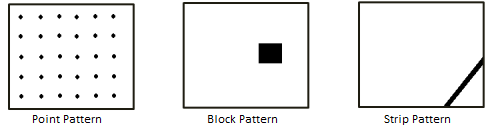
\includegraphics[width=14cm,height=5cm]{chapter5/ART_Patterns.png}
%\caption{Failure domains across input domain~\cite{chan1996proportional}}
%\label{fig:patterns}
%\end{figure}


% It is important to note that these techniques only identify a single instance of failure and do not  focus on the failure domain. 

%2.	It is also noticed that further analysis of fault lead to new faults which the testing process may not have identified.
%3. 	Experiments can be performed to analyse the frequency of existence of point, block and strip domain across the input domain. 

%Random testing is a black-box testing technique in which parts (methods/modules) of SUT are selected randomly and then executed against randomly generated test data from the whole input domain. Results obtained from the execution are either compared to the specifications of the SUT or language exceptions which served as a test oracle. Any test output that fail to meet the oracle either because of failing to comply the specification or trigger the exceptions are considered as potential faults. In this paper we present a new tool, called Automated Discovery of Failure Domain (ADFD), based on a random testing tool called York Extensible Testing Infrastructure (YETI), for not only finding fault but also its domain. ADFD utilise YETI to discover the fault in the given SUT and then generate a dynamic code for finding its domain. The found domain -- point, block or strip are presented on the graph at the end of each test session


%ADFD has been designed to decrease the time of system testing. Knowing the domain of the fault the debuggers This research can decrease the overall testing time by reducing the number of code exchanges between testers and debugger. It is achieved by tracking the failure domain and not only a single instance failure. Tracking failure domain provide more information about the behaviour of the fault.

%that also served as regression testing. None of the testing techniques evaluate the nature of the fault and the pattern in which the fault reside. 


%The aim of this research study is to find not only find the values for which the system fails but also the domains of failure causing inputs which will help in automated generation of fault targeted test cases for any black-box testing technique.\\


%Over the past few years there is a tremendous growth in development of hardware whose main focus is to increase the computer processing power. The computers that served as a mini and mainframe computers few years ago are turned into personal computer in todays modern age. To utilise this processing power various software development companies started to develop more sophisticated and processing hungry softwares. These softwares provide simple and easy to use Graphical User Interface (GUI) but on the back end they are equally complex and consist of thousands of instructions. This increase in size of the software also increases the difficulty of preserving high quality, reliability, portability, maintainability and efficiency of the software. These problems are mainly cater by software testing. The increase of complexity and size of softwares also forced the researchers to find new ways of software testing that are more efficient, reliable and speedy to cope with the ever increasing hardware and software industry.\\

%Mirror Adaptive Random Testing (MART) ~\cite{Chen2003}, Feedback-directed Random Testing (FDRT)~\cite{Pacheco2007}, Restricted Random Testing (RRT)~\cite{Chan2002} and Quasi Random Testing  (QRT)~\cite{Chen2005} are the strategies based on the same principle that found better results compared to ordinary random testing.

The Adaptive Random Testing (ART), Restricted Random Testing (RRT)~\cite{chan2006restricted}, Mirror Adaptive Random Testing (MART) ~\cite{chen2004mirror}, Adaptive random testing for object oriented program (Artoo)~\cite{ciupa2008artoo}, Directed Adaptive Random Testing (DART) ~\cite{godefroid2005dart}, Lattice-based Adaptive Random Testing (LART)~\cite{mayer2005lattice} and Feedback-directed Random Testing (FDRT)~\cite{pacheco2007randoop, pacheco2007feedback} are few of the improved versions of random testing based on the existence of contiguous failure domains within the input domain (see Section~\ref{sec:failuredomains_2} for more details). All these techniques tries to detect a single instance of failure ignoring the underlying failure domain. It is interesting that, in our knowledge, no specific strategy has been developed to evaluate the failure domains. This chapter describes a new test strategy called Automated Discovery of Failure Domain (ADFD), which not only finds the failure and failure domains but also present the pass and fail domains graphically. The idea of identification of pass and fail domain is attractive because it provides an insight of the domains in the given SUT. Some important aspects of ADFD strategy presented in the chapter include:

\begin{itemize}
\item Description and implementation of the new ADFD strategy in YETI.
\item Evaluation to assess ADFD strategy by testing classes with different failure domains.
\item Reduction in test duration by identification of all failure domains instead of a single instance of failure.
\item Improvement in test efficiency by helping debugger to consider all failure occurrences during debugging. 
\end{itemize}


% Additionally, ADFD test strategy can also be used to identify frequency of point, block and strip fault domain across the production softwares.



%The main objective behind ADFD is to get an automated frame work that find the existence of fault and fault domain across the input domain, decrease debugging time and to discover any more faults missed by the testing system. Significant research has been done to utilise the failure domains but their existence, nature and boundaries need further attention. Having fault domain information prior to testing enables the tester to guide testing according to the failure domain of the SUT, for example pure random testing is more effective for point domain than block and strip domains where as ART, MART, FDRT, RRT and QRT are more effective for block and strip fault domains than point fault domain.

%In our previous research we extended the same idea of the existence of different domains of failure across the whole input domain proposed by Chen et al,~\cite{Chen2008} and accepted by various other researchers to develop a new strategy called Dirt Spot Sweeping Strategy [X]. However the experimental results showed not very considerable improvement then what we predicted. We performed 500 experiments in which we carried out 10000 tests but the results showed only 5\% improvement contrary to our prediction of 30\%. All the experiments were performed from a pool of open-source projects bundled in a repository called Qualitas Corpus~\cite{Tempero2010}. Corpus contains more than 100 open-source java projects and maintained only for the purpose of unbiased research experiments. Therefore one of the conclusions derived from our experiments was that the patterns of failure may not exist in most of the software’s due to which our strategy which focus on these patterns didn’t produce much efficiency.\\
%It was therefore very interesting for us to do further research to find about the existence and nature of these failure patterns. Our main focus in this research paper is to discover whether there exist failure patterns across the input domain or not and if they exist then how frequent and what pattern they follow.\\

%The rest of this paper is organized as follows: \\ Section~\ref{sec:adfd} describes the ADFD strategy. Section~\ref{sec:implementation} presents implementation of the ADFD strategy. Section~\ref{sec:experimentalResults} explains the experimental results. Section~\ref{sec:discussion4} discusses the results. Section~\ref{sec:validity} presents the threats to validity. Section~\ref{sec:relatedWork} presents related work and Section~\ref{sec:conclusion}, concludes the study.

%In Section II, we describe the automated discovery of failure domain test strategy and explain its structure and function with the help of a flowchart and motivating example. Section III presents its implementation in automated random testing tool called York Extensible Testing Infrastructure (YETI). Section IV and V report the experiments performed using the proposed technique and evaluate \& discuss the obtained results. Section VI and VII discuss any threats to validity and related discussion. Finally we conclude in Section VIII. 

%The rest of this paper is organized as follows. The sections, II to X, describe automated strategy, Implementation, Experimental setup and analysis, Evaluation, Experimental results, discussion, conclusion and future work respectively.\\

%X\section{Problems and Solutions}\label{sec:probl_and_sol}
%This paper address five. main problems in random testing. These are (1) Finding the whole domain of fault instead of only failing values, (2) Representation of fault values, (3) automation of the evaluation process, (4) Identification of fault domain for multi arguments methods and its representation, (5) Generation and classification of test values for Strings and complex (non scaler) arguments. This section elaborate each of the above mention problem and describe our proposed solution (if any) to them.

%\subsection{Finding the whole domain of fault instead of only failing values}
%Most of the testing tools take into account only the fault finding values with out giving due consideration to the domain in which the values exist. \subsection{Representation of fault values and fault domains}
%points: instead of dumping logs and more complex reports we describe the fault domains with the help of charts. 
%\subsection{Automation of the testing process}
%We developed an automated system to test the system, generate the fault domain finding files, compile and execute them to find the fault domains if any. points: automation is achieved by combining the test tool and evaluation system e.g. yeti and ADFD.   
%\subsection{Identification and representation of multi arguments data}
%I think it is beyond the scope of this study to identify and represent more then 3 arguments method because at the moment we can show only three diminutional charts.
%\subsection{Generation and classification of test values for string and complex (non scaler) arguments}
%It is difficult to find the domain for strings and complex (non scaler) data therefore they can be exempted from this study.


\section{Automated Discovery of Failure Domain}\label{sec:adfd}

Automated Discovery of Failure Domain (ADFD) strategy is proposed as the improvement on R$^+$ strategy with capability of finding failures as well as the failure domains. The output produced at the end of test session is a chart showing the passing value or range of values in blue and failing value or range of values in red. The complete work flow of ADFD strategy is given in Figure \ref{fig:ADFD-workflow}.

The process is divided into five major steps given below, and each step is briefly explained in the following paras.

\begin{enumerate}
\item GUI front-end for providing input
\item Automated finding of failure
\item Automated generation of modules
\item Automated compilation and execution of modules to discover domains
\item Automated generation of graph showing domains
\end{enumerate}

\bigskip
\begin{figure}[ht]
\centering
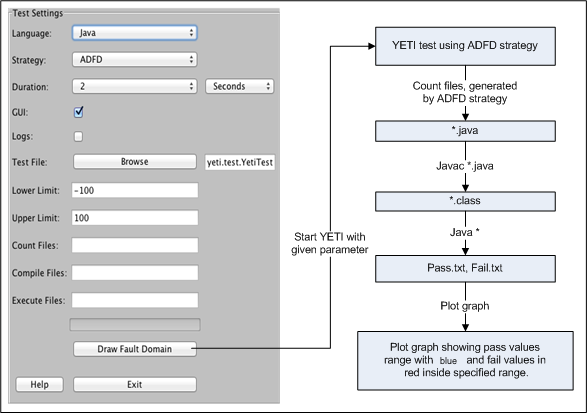
\includegraphics[width=15cm,height=11cm]{chapter5/ADFD_Diagram1.png}
\bigskip
\caption{Work flow of ADFD strategy}
\label{fig:ADFD-workflow}
\end{figure}
\bigskip

\subsection{GUI front-end for Providing Input:}
ADFD strategy is provided with an easy to use GUI front-end to get input from the user. It takes YETI specific input, including program language, strategy, duration, enable or disable YETI GUI, logs and program in byte code. In addition, it also takes minimum and maximum values to search for failure domain in the specified range. Default range for minimum and maximum is taken as Integer.MIN\_INT and Integer.MAX\_INT respectively. The GUI front-end of ADFD technique is given in Figure~\ref{fig:ADFD-frontend}.


\subsection{Automated Finding of Failure:}
ADFD, being extended form of R$^+$ strategy, relies on R$^+$ strategy to find the first failure. Random$^+$ strategy is an improvement on random strategy with preference for the boundary values to provide better failure finding ability. % ADFD strategy is implemented in YETI which is famous for its simplicity, high speed and proven ability of finding potentially hazardous faults in many systems~\cite{Oriol2011, Oriol2012}. YETI is quick and can call up to one million instructions in one second on Java code. It is also capable of testing VB.Net, C, JML and CoFoJa beside Java. \\

\subsection{Automated Generation of Modules:}
After a failure is found in the SUT, ADFD strategy generates complete new Java program to search for failure domains in the given SUT.  These programs with ``.java" extensions are generated through dynamic compiler API included in Java 6 under javax.tools package. The number of programs generated can be one or more, depending on the number of arguments in the test module i.e. for module with one argument one program is generated, for module with two arguments two programs and so on. To track failure domain, the program keeps only one argument as variable and the remaining arguments as constant in the program generated at run time.

\begin{figure}[H]
\begin{center}
%\centring
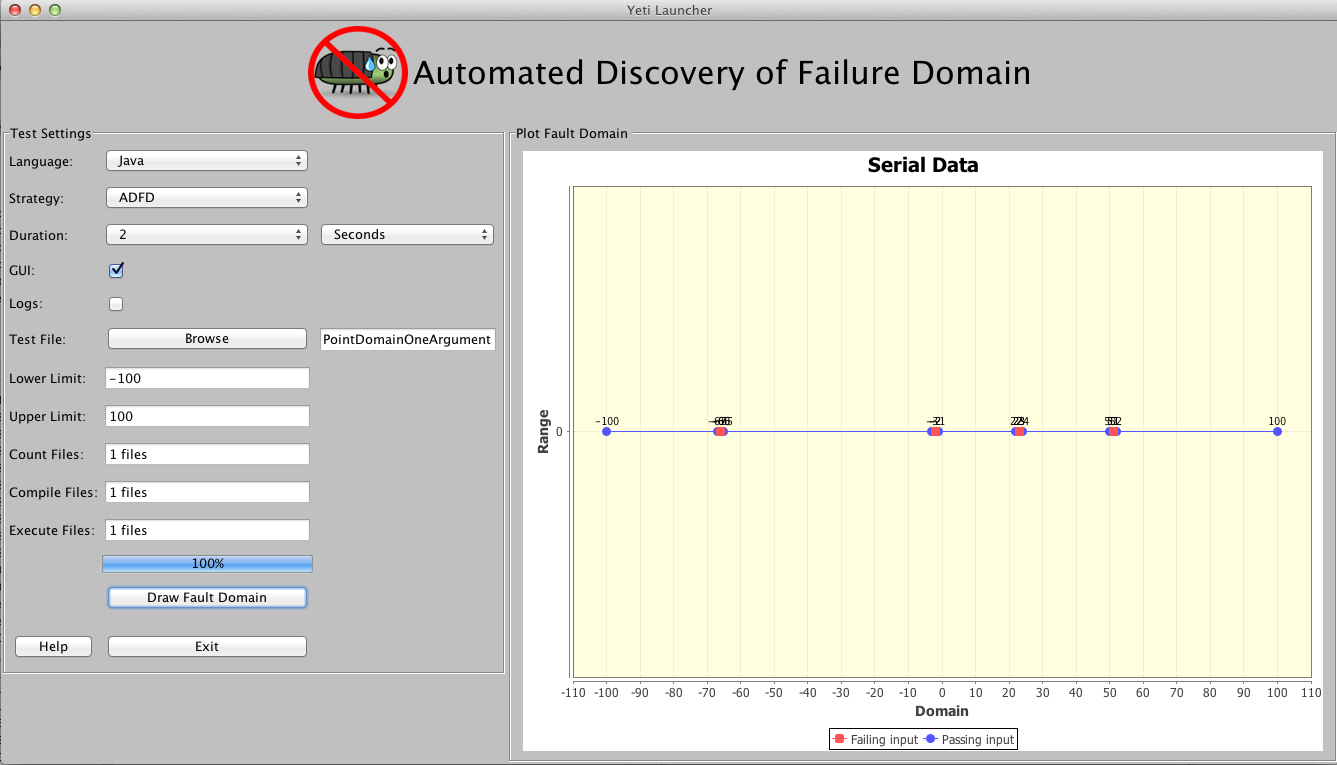
\includegraphics[width=15cm,height=11cm]{chapter5/ADFD_front_end.png}
\bigskip
\caption{Front-end of ADFD strategy}
\label{fig:ADFD-frontend}
\end{center}
\end{figure}

\subsection{Automated Compilation and Execution of Modules:}
The java modules generated in the previous step are compiled using $javac~*$ command to get their binary $.class$ files. The $java~*$ command is applied to execute the compiled programs. During execution, the constant arguments of the module remain the same but the variable argument receives all the values ranging, from minimum to maximum, specified at the beginning of the test. After execution is completed we get two text files of $Pass.txt$ and $Fail.txt$. Pass file contains all the values for which the modules behave correctly while fail file contains all the values for which the modules fail.

\subsection{Automated Generation of Graph:}
The values from the pass and fail files are used to plot (x, y) chart using JFreeChart~\cite{gilbert2008jfreechart}. JFreeChart is a free open-source java library that helps developers to display complex charts and graphs. Lines and circles with blue colour represent pass values while lines and squares with red colour represents fail values. Resultant graph clearly depicts both the pass and fail domain across the specified input domain. The graph shows red points when the program fails for only one value, blocks when the program fails for multiple values and strips when the program fails for a long range of values.%\subsection{Flow Chart of the process}

%The following flow chart clearly identify the workflow of the whole process and the various steps involved in the process.

%\begin{figure}[p]
%\centering
%\includegraphics[width=8cm,height=12cm]{automatedFail.png}
%\caption{Automated discovery of Failure Domain}
%\label{fig:autofail}
%\end{figure}




%We found that it is better for the developer to see the range because the fault can be found once but it can generate errors at multiple locations.like point pattern in the first graph only generate fault at location 0 but if the same zero is assigned to second argument then the whole domain values can fail.\\


%\begin{figure}[htp]
%\centering
%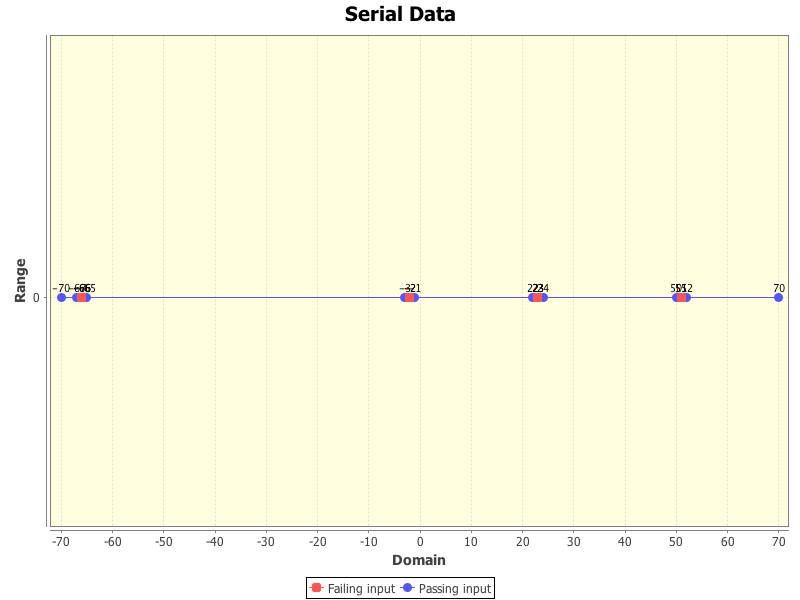
\includegraphics[width=8.5cm,height=6cm]{oneArgumentPointDomain.png}
%\caption{Point pattern failure domain}
%\label{fig:patterns}
%\end{figure}


%Figure \ref{fig:point} shows the example of point pattern. In sub figure \ref{fig1:a} test only fails for 0 out of the whole integer range where as in sub figure \ref{fig1:b} all test fails when static variable is assigned with 0 value.


%\begin{figure}[htp]
%\centering
%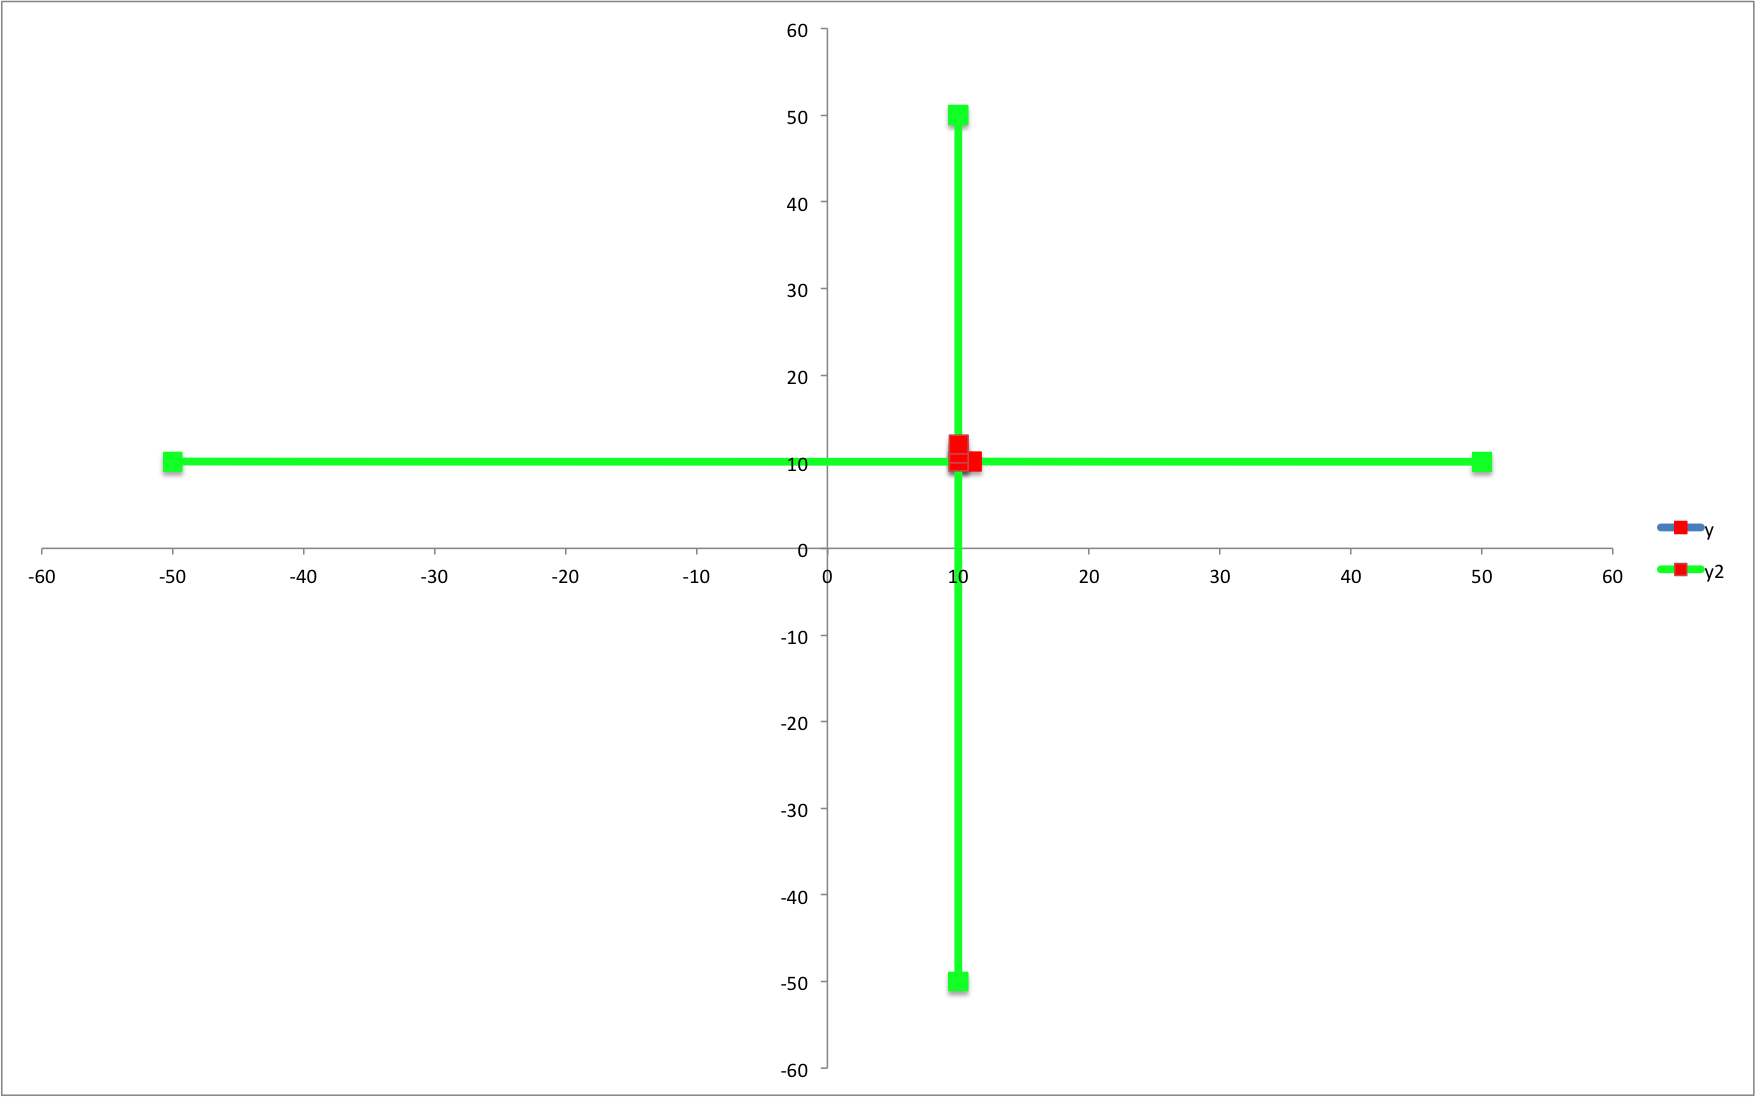
\includegraphics[width=4cm,height=4cm]{block_pattern.png}
%\caption{Block pattern failure domain}
%\label{fig:patterns}
%\end{figure}


%Figure \ref{fig:block} shows the example of block pattern. Both sub figure \ref{fig1:a} and \ref{fig1:b} shows the block pattern of failure. The failure values are given in table \ref{tb:failtable}.

%\begin{figure}[htp]
%\centering
%\begin{center}
%  % Maximum length
 %\subfloat[Test 1 A]{\label{fig1:a}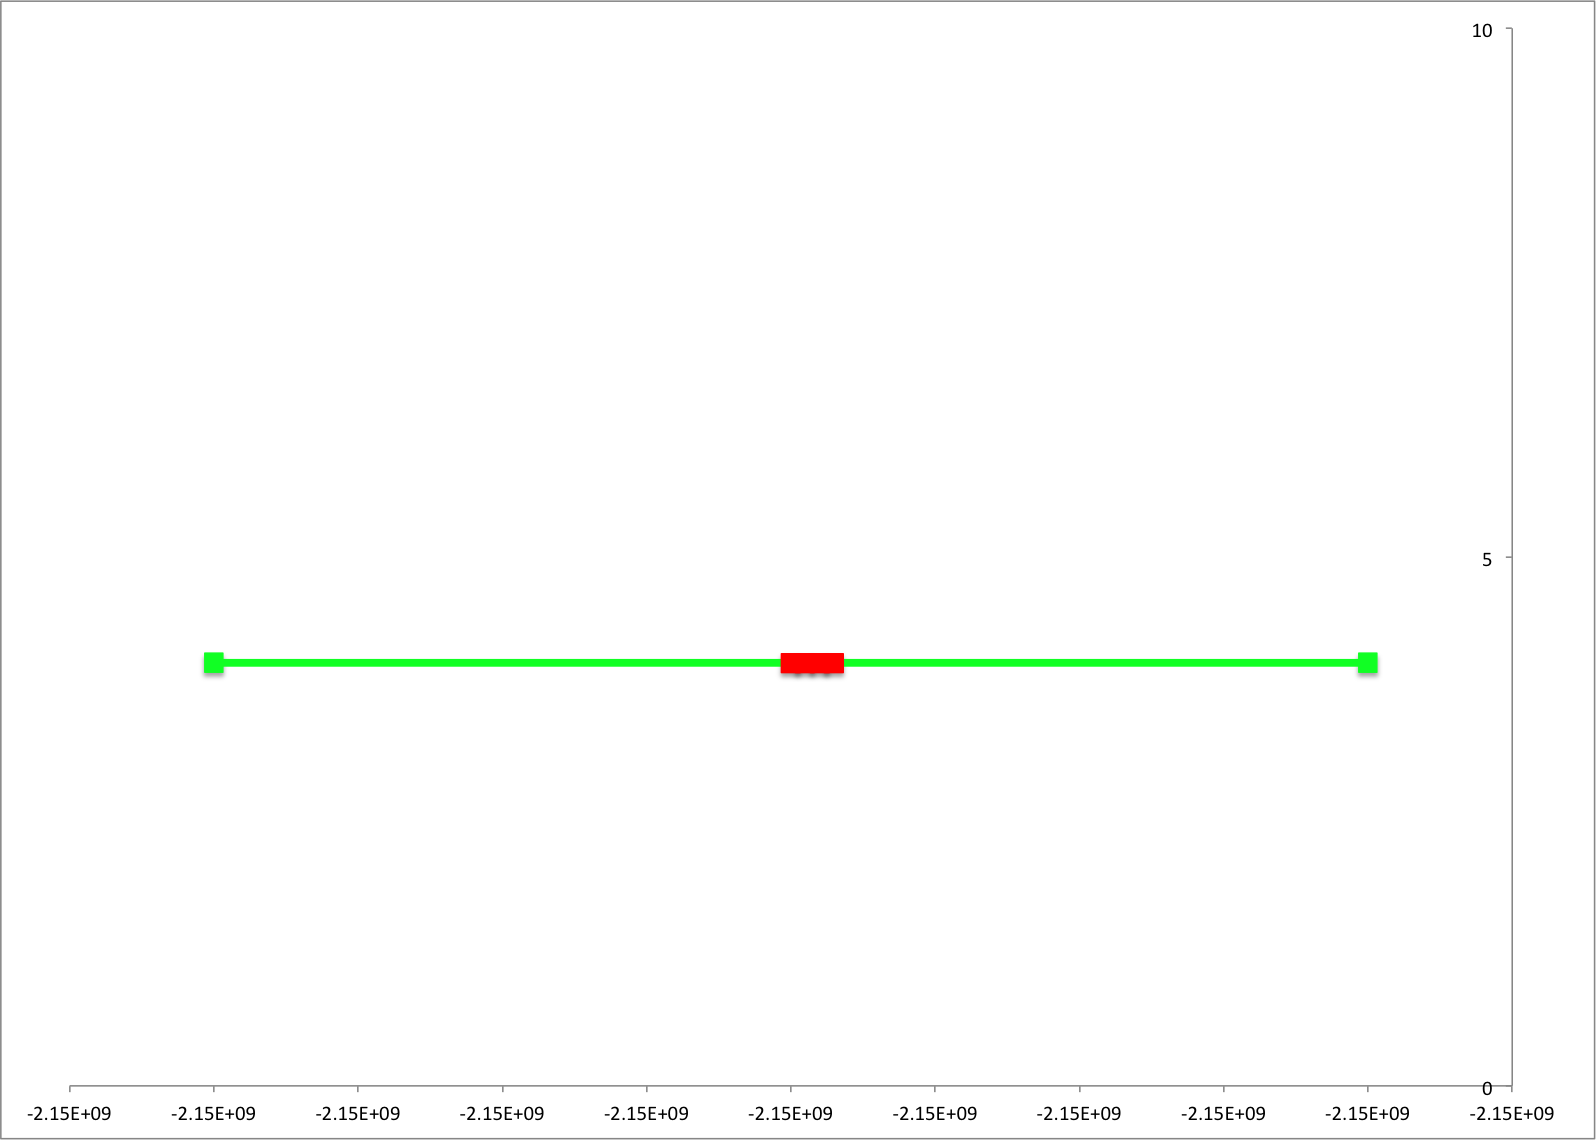
\includegraphics[width=0.49\linewidth]{excel_png/strip_pattern_B.png}}\hfill
 %\subfloat[Test 1 B]{\label{fig1:b}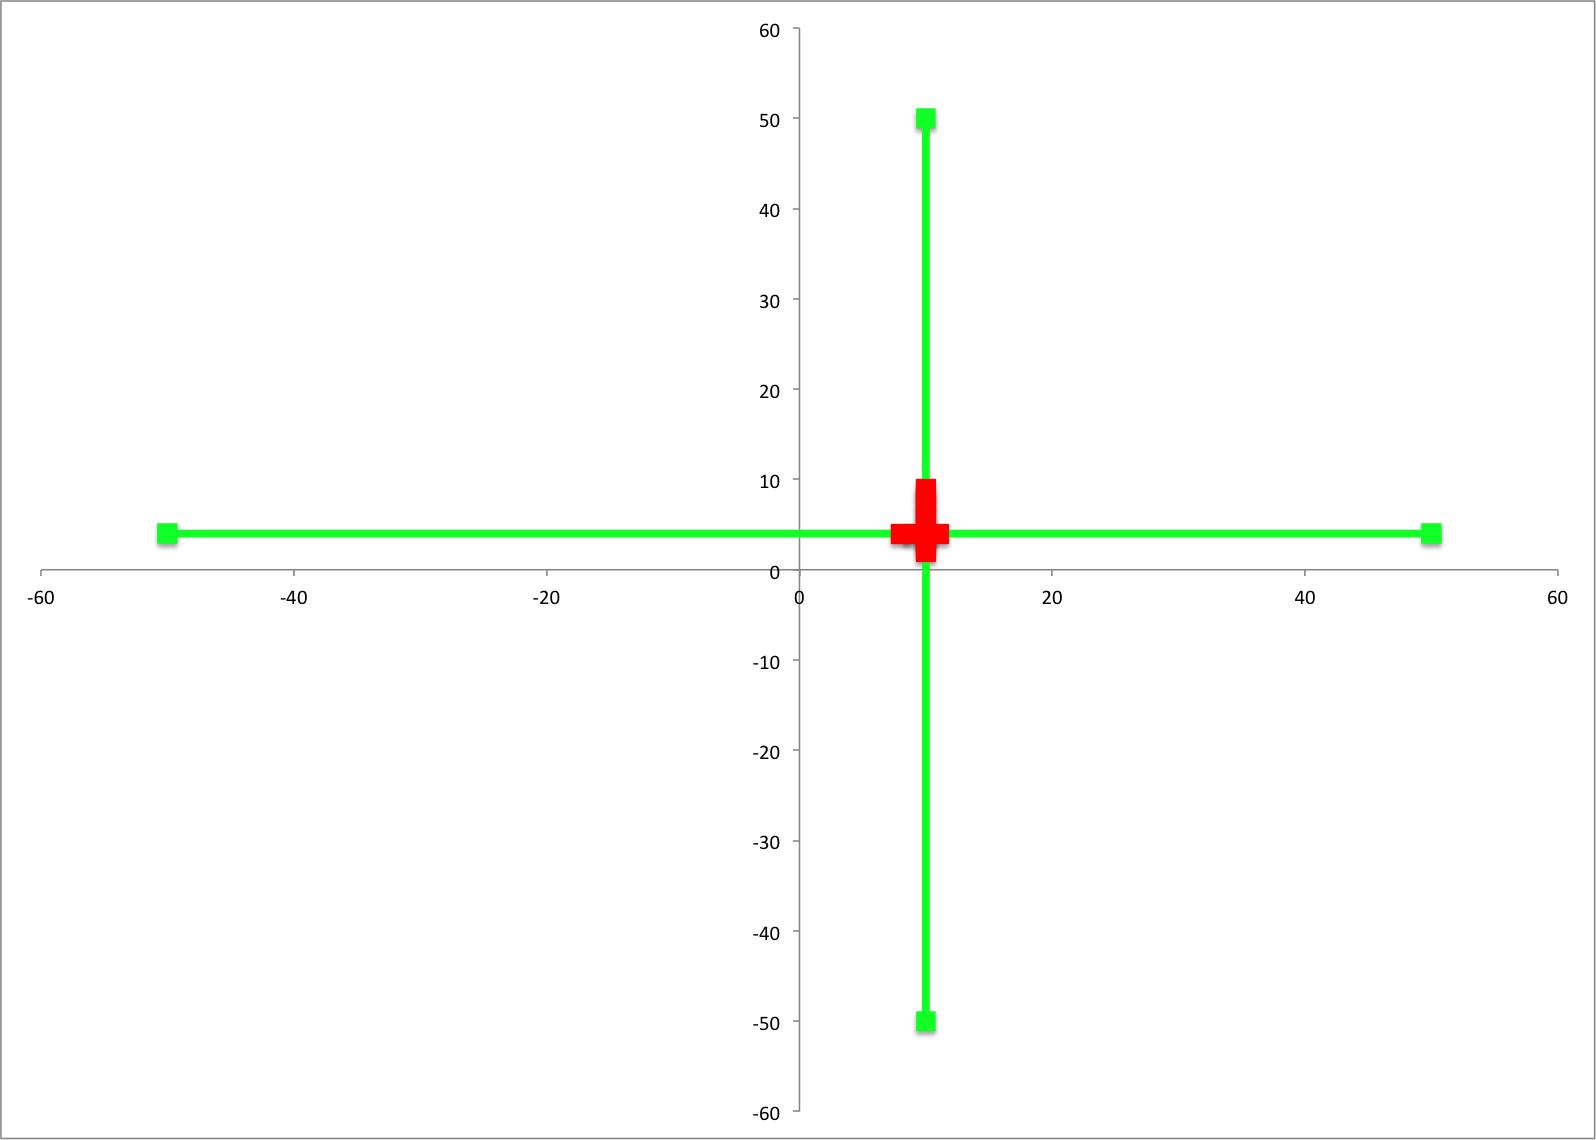
\includegraphics[width=0.49\linewidth]{excel_png/strip_pattern_A.png}}
%  end{center}
%\caption{Strip pattern failure domain}
%%  \label{fig:strip}
%\end{figure}

%Figure shows the example of strip pattern. Here we have two strip failure pattern for test 1 shown in \ref{fig1:a} and \ref{fig1:b} while 1 other for test 2 given in . The failure values are given in table .\\

\section{Implementation}\label{sec:implementation}
The ADFD strategy is also implemented in YETI. Please refer to Chapter~\ref{chap:yeti_3} for details on YETI. In this section, we give a brief overview of the implementation of ADFD strategy in YETI and illustrate it with the help of an example. 
\bigskip
\begin{figure}[h]
\centering
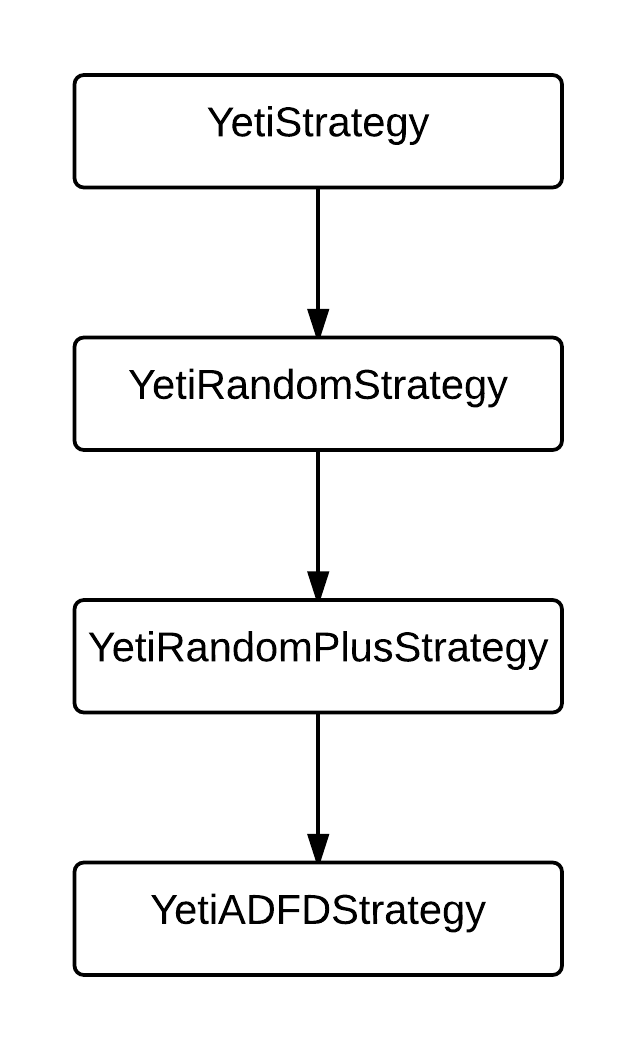
\includegraphics[width=6cm,height=8cm]{chapter5/classHierarchy2.png}
\caption{Class Hierarchy of ADFD strategy in YETI}
\label{fig:hierarchyofADFD}
\end{figure}
%\subsection{York Extensible Testing Infrastructure}
%YETI is a testing tool developed in Java that tests programs using random strategies in an automated fashion. YETI meta-model is language-agnostic which enables it to test programs written in functional, procedural and object-oriented languages.

%YETI consists of three main parts including core infrastructure for extendibility through specialisation, strategies section for adjustment of multiple strategies and languages section for supporting multiple languages. Both the languages and strategies sections have a pluggable architecture to easily incorporate new strategies and languages making YETI a favourable choice to implement ADFD strategy. YETI is also capable of generating test cases to reproduce the failures found during the test session.
 
 \subsection{ADFD strategy in YETI}
ADFD strategy is implemented in the strategies section of YETI. This section contains various strategies including random, random$^+$ and DSSR to be selected for testing according to the specific needs. The default strategy for testing YETI is random. On top of the hierarchy in strategies section, is an abstract class YetiStrategy, which is extended by YetiRandomStrategy and it is further extended to get YetiRandomPlusStrategy. YetiADFDStrategy is developed by extending the YetiRandomPlusStrategy.



% as shown in figure \ref{fig:hierarchy}. 
 
%\begin{figure}[h]
%\centering
%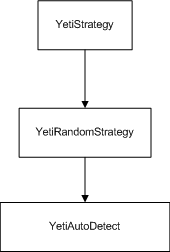
\includegraphics[width=3cm,height=3.5cm]{Hierarchy1.png}
%\caption{Class Hierarchy of automated discovery of failure domains in YETI}
%\label{fig:hierarchy}
%\end{figure}

\subsection{Example}\label{sec:example}
For a concrete example to show how ADFD strategy in YETI proceeds, we suppose YETI tests the following class with ADFD strategy selected for testing. Note that for more clear visibility of the output graph generated by ADFD strategy at the end of test session, we fix the values of lower and upper range by -70 and 70 from Integer.MIN\_INT and Integer.MAX\_INT. 

\begin{lstlisting}
/**
 * Point Fault Domain example for one argument program
 * @author (Mian and Manuel)
 */
public class PointDomainOneArgument{
	public static void pointErrors (int x){
 		if (x == -66) 
			 	abort(); 		/* error */
		if (x == -2) 
			 	abort(); 		/* error */
 		if (x == 51) 
			 	abort(); 		/* error */
		if (x == 23) 
			 	abort(); 		/* error */
	}
}
\end{lstlisting}

%Published programs from literature~\cite{Chen2003}\cite{Chan1996}\cite{Chen2004} of point, block and strip failure patterns are tested to explain the working of ADFD . These programs were translated in to java language for this experiment (See appendix 1 for more details). 

\begin{figure}[H]
\centering
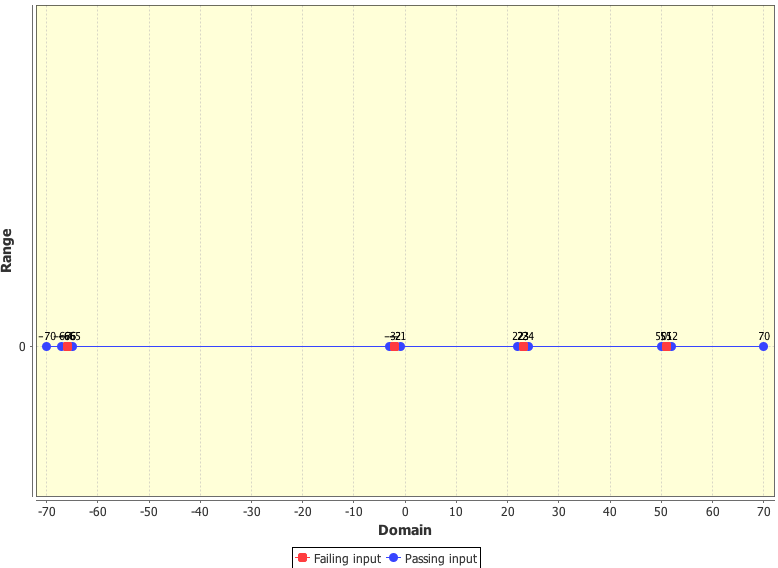
\includegraphics[width=12.2cm,height=8cm]{chapter5/pointDomainOneArgument.png}
\caption{ADFD strategy plotting pass and fail domain of a given class}
\label{fig:ADFD-example}
\end{figure}

As soon as any one of the above four failures are discovered the ADFD strategy generates a dynamic program given in Appendix \ref{sec:appendix1} (7). This program is automatically compiled to get the binary file and then executed to find the pass and fail domains inside the specified range. The identified domains are plotted on a two-dimensional graph. It is evident from the output presented in Figure \ref{fig:ADFD-example} that ADFD strategy not only finds all the failures but also plots the pass and fail domains.


\begin{comment}
%%%%%% They are commented in this format to decrease the text, for two column format uncomment them.

%ADFD can be activated by typing the command java -jar ADFD.jar. After the GUI of ADFD is launched we need to specify yeti specific values that include language of the program under test, strategy for the current test session, duration of test session (minutes or milli-second), display YETI GUI or not and display real time logs or not. Next we browse to select the file for testing and the run button starts testing the file with YETI. 

\bigskip
\begin{figure}[ht]
\centering
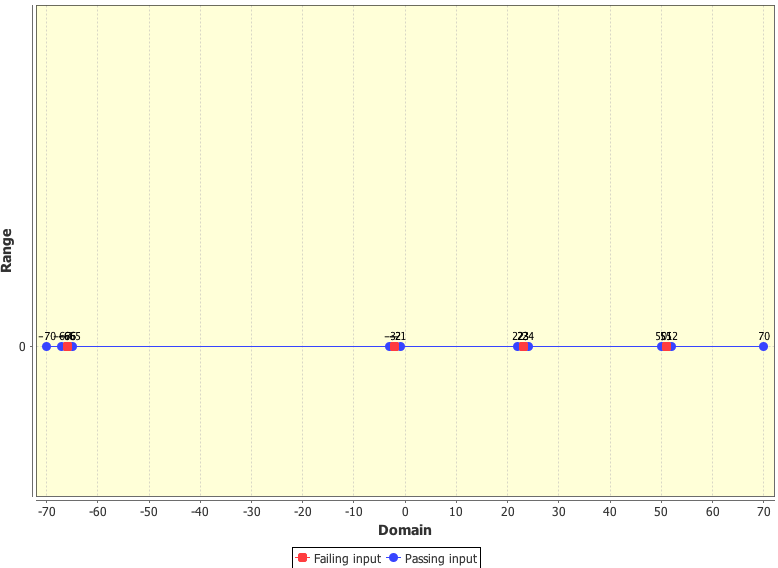
\includegraphics[width=12.2cm,height=8.5cm]{chapter5/pointDomainOneArgument.png}
\bigskip
\caption{ADFD strategy plotting pass and fail domains of the given class}
\label{fig:ADFD-plot}
\end{figure}
\bigskip

%In 5 second YETI found one fault out of the above 4 faults. The ADFD strategy in YETI generate a source file (C*.java) at the end of the test session. This file contain the code that searches for fault domains. The count button count the number of files. ADFD create the number of files on the basis of the number of arguments in the method under test. For one argument one method is created and for two argument two methods are created. 

%The next button is compile which compile the generated files and generate the byte code (.class files). The execute button execute the byte code and test the method under test for all the values between upper and lower bound. At the end of execution it generates two files (pass.txt and fail.txt). Pass file contain all the values for which the method performed correctly while fail file contain all the values for which the method under test fail.

%The draw fault domain button reads the pass and fail files and plot them on the x, y graph where red line with squares show the failing values while the blue line with square shapes show the passing values.
\end{comment}

%%%%%%%%%%%%%%%%%%%%%%%%%%%%%%%%%%%%%%%%%%%%%%%%%%%%%%%%

\section{Experimental Results} \label{sec:experimentalResults}
This section includes the experimental set-up and results obtained by using ADFD strategy. Six numerical programs of one and two-dimension were selected. These programs were error-seeded in such a way to get all the three forms of point, block and strip domains. Each selected program contained various combinations of one or more failure domains. 

All experiments were performed on a 64-bit Mac OS X Lion Version 10.7.5 running on 2 x 2.66 GHz 6-Core Intel Xeon with 6.00 GB (1333 MHz DDR3) of RAM. YETI runs on top of the Java\texttrademark  SE Runtime Environment [version 1.6.0\_35]. 

To elucidate the results, six programs were developed so as to have separate program for one and two-dimensional point, block and strip failure domains. The code of the selected program is given in Appendix \ref{sec:appendix1} (1-6). The experimental results are presented in Table \ref{table:failtable} followed by description under three headings.
%To elucidate the results, six programs were developed so as to have separate program for one and two-dimension point, block and strip fault domains. The code of selected programs is given in Appendix \ref{sec:appendix1} (2-7). The experimental results are presented in Table \ref{table:failtable} and described under the following three headings.
%\begin{center}

%\end{center}
\bigskip
\begin{table}[h]
%\renewcommand{\arraystretch}{2}
\caption{Experimental results of programs tested with ADFD strategy}
\bigskip
\centering
{\renewcommand{\arraystretch}{1.3}
\scriptsize
%\normalsize

\begin{tabular}{|c|c|c|l|l|l|}

\hline 


\multirow{2}{*}{S.No}	& \multirow{2}{*}{Fault }	 				& \multirow{2}{*}{Module} 		& \multirow{2}{*}{Specific Fault}	 		& \multirow{2}{*}{Pass Domain} 					& \multirow{2}{*}{Fail Domain} 			\\  
					& Domain								&  Dimension					&									&											&								\\ \hline 
\multirow{6}{*}{1} 	&	\multirow{6}{*}{Point}				& 	\multirow{3}{*}{One}			&	\multirow{3}{*}{PFDOneA(i)}	&	-100 to -67, -65 to -3, 		  		& -66, -2, 23, 51			 	\\  
				&									&							&							&	-1 to 50, 2 to 22, 					&							\\  
				&									&							&							&	24 to 50, 52 to 100					&							\\ \cline{3-6}
				&									&	\multirow{3}{*}{Two}			&	\multirow{2}{*}{PFDTwoA(2, i)}	&	(2, 100) to (2, 1),	 				&  (2, 0)						\\  
				&									&							&							&	(2, -1) to (2, -100)					&							\\ \cline{4-6}
				&									& 							&	PFDTwoA(i, 0)				&	Nil								& (-100, 0) to (100, 0)				\\  \hline



\multirow{5}{*}{2} 	&	\multirow{5}{*}{Block}				& 	\multirow{2}{*}{One}			&	\multirow{2}{*}{BFDOneA(i)}	&	-100 to -30, -25 to -2, 					& 	-1 to 1, -29 to -24,		 	\\ 
				&									&							&							&	2 to 50, 55 to 100						&	51 to 54,				\\   \cline{3-6}
				&									&	\multirow{3}{*}{Two}			&	\multirow{2}{*}{BFDTwoA(-2, i)}	&	(-2, 100) to (-2, 20), 					& 	(-2 , 1) to ( -2, 19), 		\\ 
				&									&							&							&      (-2, -1) to (-2, -100)					&	(-2, 0)				\\ \cline{4-6}
				&									& 							&	BFDTwoA(i, 0)				&	Nil								& 	(-100, 0) to (100, 0)		\\  \hline
				
				



\multirow{5}{*}{3} 	&	\multirow{5}{*}{Strip}					& 	\multirow{2}{*}{One}			&	\multirow{2}{*}{SFDOneA(i)}	&	\multirow{2}{*}{-100 to -5, 35 to 100}		& 	\multirow{2}{*}{-4, 34	}\\ 
				&									&							&							&									&				\\  \cline{3-6}
				&									&	\multirow{3}{*}{Two}			&	\multirow{2}{*}{SFDTwoA(-5, i)}	&	(-5, 100) to (-5, 40),					&  (-5, 39) to (-5, 1), 			\\ 
				&									&							&							&	 (-5, 0) to (-5, -100)					&	(-5, 0)				\\ \cline{4-6}
				&									& 							&	SFDTwoA(i, 0)				&	Nil								&  (-100, 0) to (100, 0)			\\  \hline
				
				
\end{tabular}
}
\label{table:failtable}
\end{table}

\bigskip

\textbf{Point Failure Domain:}  Two separate Java programs Pro1 and Pro2, given in Appendix \ref{sec:appendix1} (1, 2), were tested with ADFD strategy in YETI to get the findings for point failure domain in one and two-dimension program. Figure \ref{fig:PFDOne} presents range of pass and fail values for point failure domain in one-dimension whereas Figure \ref{fig:PFDTwo} presents range of pass and fail values for point failure domain in two-dimension program. The range of pass and fail values for each program in point failure domain is given in Table \ref{table:failtable}.
%%%%%%%%%%%%%%%%Point Domain%%%%%%%%%%%%%%%%%%%%%%%%%%%%%

\begin{figure} [H]
\centering
\subfigure[One dimension module]{
\includegraphics[width=15cm,height=7.5cm]{chapter5/PFDOne.png}
\label{fig:PFDOne}
}

\bigskip
\subfigure[Two dimension module]{
\includegraphics[width=15cm,height=7.5cm]{chapter5/PFDTwo.png}
\label{fig:PFDTwo}
}
\bigskip
\caption{Chart generated by ADFD strategy presenting point failure domain}
\end{figure}
\bigskip
%\begin{figure}[H]
%\centering
%\includegraphics[width=8.2cm,height=5cm]{PFDOne.png}
%\caption{Chart generated by ADFD strategy presenting point fault domain in one dimension module}
%\label{fig:PFDOne}
%\end{figure}

%\begin{figure}[H]
%\centering
%\includegraphics[width=8.2cm,height=5cm]{PFDTwo.png}
%\caption{Chart generated by ADFD strategy presenting point fault domain in two dimension module}
%\label{fig:PFDTwo}
%\end{figure}

\newpage
\noindent \textbf{Block Failure Domain:}  Two separate Java programs Pro3 and Pro4 given in Appendix \ref{sec:appendix1} (3, 4) were tested with ADFD strategy in YETI to get the findings for block failure domain in one and two-dimensional program. Figure \ref{fig:BFDOne} presents a range of pass and fail values for block failure domain in one-dimension whereas Figure \ref{fig:BFDTwo} presents a range of pass and fail values for block failure domain in two-dimension program. The range of pass and fail values for each program in block failure domain is given in Table \ref{table:failtable}.
%%%%%%%%%%%%%%%Block domain %%%%%%%%%%%%%%%%%%%%%%%%%%%%%%
%%%





\begin{figure} [H]
\centering
\subfigure[One dimension module]{
\includegraphics[width=15cm,height=7.5cm]{chapter5/BFDOne.png}
\label{fig:BFDOne}
}
\bigskip

\subfigure[Two dimension module]{
\includegraphics[width=15cm,height=7.5cm]{chapter5/BFDTwo.png}
\label{fig:BFDTwo}
}
\bigskip
\caption{Chart generated by ADFD strategy presenting block failure domain}
\end{figure}


%\begin{figure}[H]
%\centering
%\includegraphics[width=8.2cm,height=5cm]{BFDOne.png}
%\caption{Chart generated by ADFD strategy presenting block fault domain in one dimension module}
%\label{fig:BFDOne}
%\end{figure}


%\begin{figure}[H]
%\centering
%\includegraphics[width=8.2cm,height=5cm]{BFDTwo.png}
%\caption{Chart generated by ADFD strategy presenting block fault domain in two dimension module}
%\label{fig:BFDTwo}
%\end{figure}


\newpage
\noindent \textbf{Strip Failure Domain:} Two separate Java programs Pro5 and Pro6 given in Appendix \ref{sec:appendix1} (5, 6) were tested with ADFD strategy in YETI to get the findings for strip failure domain in one and two-dimension program. Figure \ref{fig:SFDOne} presents range of pass and fail values for strip failure domain in one-dimension whereas Figure \ref{fig:SFDTwo} presents a range of pass and fail values for strip failure domain in two-dimension program. The range of pass and fail values for each program in strip failure domain is given in Table \ref{table:failtable}.


%
%%%%%%%%%%%%%%%%%%%%%%Strip domain %%%%%%%%%%%%%%%%%%%%%%%
\begin{figure} [H]
\centering
\subfigure[One dimension module]{
\includegraphics[width=15cm,height=7.5cm]{chapter5/SFDOne.png}
\label{fig:SFDOne}
}
\bigskip
\subfigure[Two dimension module]{
\includegraphics[width=15cm,height=7.5cm]{chapter5/SFDTwo.png}
\label{fig:SFDTwo}
}
\bigskip
\caption{Chart generated by ADFD strategy presenting Strip failure domain}
\end{figure}






%\begin{figure}[H]
%\centering
%\includegraphics[width=8.2cm,height=5cm]{SFDOne.png}
%\caption{Chart generated by ADFD strategy presenting strip fault domain in one dimension module}
%\label{fig:SFDOne}
%\end{figure}

%\begin{figure}[H]
%\centering
%\includegraphics[width=8.2cm,height=5cm]{SFDTwo.png}
%\caption{Chart generated by ADFD strategy presenting strip fault domain in two dimension module}
%\label{fig:SFDTwo}
%\end{figure}



\section{Discussion} \label{sec:discussion4}

ADFD, with a simple graphical user interface, is a fully automated testing strategy which identifies failures, failure domains and visually present the pass and fail domains in the form of a chart. Since all the default settings are set to the optimum level, the user needs only to specify the module to be tested and click ``Draw fault domain" button to start test execution. All the steps including Identification of fault, generation of dynamic java program to find domain of the identified failure, saving the program to a permanent media, compiling the program to get its binary, execution of binaries to get pass and fail domain and plotting these values on the graph are done completely automatically without any human intervention.

As evident from the results, ADFD strategy effectively identified failures and failure domains in selected programs. Identification of the failure domain is simple for one and two-dimensional numerical program but as the dimension increases the process gets more and more complicated. Moreover, no clear boundaries are defined for non-numerical data, therefore, it is not possible to plot domains for non-numerical data unless some boundary criteria are defined.

ADFD strategy initiates testing with random$^+$ strategy to find the failure and later switches to brute-force strategy to apply all the values between upper and lower bounds for finding pass and failure domains. It was found that failures at boundary of the input domain usually passes unnoticed through random test strategy but not through ADFD strategy because it scans all the values between lower and upper bounds.


The overhead in terms of execution time associated with ADFD strategy is dependent mainly on the lower and upper bounds. If the lower and upper bounds are set to the maximum range (i.e. minimum for int is Integer.MIN\_INT and maximum Integer.MAX\_INT) then the test duration is also maximum. It is rightly so because for identification of the failure domain the program is executed for every input available in the specified range. Similarly increasing the range also shrinks the produced graph making it difficult to identify clearly point, block and strip domains unless they are of considerable size. Test duration is also influenced by identification of the first failure and the complexity of the module under test.

ADFD strategy can help the debuggers in two ways. First, it reduces the `to' and `from' movement of the program between the testers and debuggers as it identifies all the failures in one go. Second, it identifies locations of all failure domains across the input domain in a user-friendly way helping debugger to fix the fault keeping in view its all occurrences.


\section{Threats to Validity} \label{sec:validity}
The major external threat to the use of ADFD strategy on a commercial scale is the selection of a small set of error-seeded programs of only primitive types such as integer used in the experiments. However, the present study will serve as the foundation for future work to expand it to general-purpose real world production application containing scalar and non-scalar data types.

Another issue is the plotting of the objects in the form of distinctive units, because it is difficult to split the composite objects containing many fields into units for plotting. Some work has been done to quantify composite objects into units on the basis of multiple features~\cite{ciupa2006object}, to facilitate easy plotting. Plotting composite objects is beyond the scope of the present study. However, further studies are required to look into the matter in depth. 

Another threat to validity includes evaluating program with complex and more than two input arguments. In the current study, ADFD strategy has only considered scalar data of one and two-dimensions. Plotting domain of programs with complex non-scalar and more than two dimension argument is much more complicated and needs to be taken up in future studies.

Finally, plotting the range of pass or fail values for a large input domain (Integer.MIN\_INT to Integer.MAX\_INT) is difficult to adjust and does not give a clear view on the chart. To solve this problem, zoom feature was added to the strategy to magnify the areas of interest on the chart.



\section{Related Works} \label{sec:relatedWork}
Traditional random testing is quick, easy to implement and free from any bias. In spite of these benefits, the lower fault finding ability of traditional random testing is often criticised~\cite{myers2011art, offutt1996semantic}. To overcome the performance issues without compromising on its benefits, various researchers have altered its algorithm as explained in Section~\ref{sec:versionsOfRT}. Most of the alterations are based on the existence of faults and failure domains across the input domain~\cite{chan1996proportional}. 

Identification, classification of pass and fail domains and visualisation of domains have not received due attention of the researchers. Podgurski et al.~\cite{podgurski2003automated} proposed a semi-automated procedure to classify faults and plot them by using a Hierarchical Multi Dimension Scaling (HMDS) algorithm. A tool named Xslice~\cite{agrawal1995fault} visually differentiates the execution slices of passing and failing part of the test. Another tool called Tarantula uses colour coding to track the statements of a program during and after the execution of the test suite~\cite{jones2002visualization}. A serious limitation of the above-mentioned tools is that they are not fully automated and require human intervention during execution. Moreover, these tools are based on the already existing test cases whereas ADFD strategy generates test cases, discovers faults, identifies pass and fail domains and visualises them in graphical form in a fully automated manner. 


\section{Summary} \label{sec:conclusion}
Experimental results obtained by applyingADFD strategy to error-seeded numerical programs provide evidence that the strategy is highly effective in identifying the failures and plotting pass and fail domains of a given SUT. ADFD strategy can find boundary failures quickly as against the traditional random testing, which is either, unable or takes comparatively longer time to discover the failures.

The use of ADFD strategy is highly effective in testing and debugging. It provides an easy to understand test report visualising pass and fail domains. It reduces the number of switches of SUT between testers and debuggers because all the faults are identified with a single execution. It improves debugging efficiency as the debuggers keep all the instances of a fault under consideration during debugging. The strategy has the potential to be used at large scale. However, future studies are required to use it with programs of more than two-dimension and different non-scaler argument types.






% ------------------------------------------------------------------------


%%% Local Variables: 
%%% mode: latex
%%% TeX-master: "../thesis"
%%% End: 
